\section{Wishart Distribution}

\subsection{Standard Wishart distribution}

the pdf of the Wishart is

\begin{equation}
	f(x; n,p,V) = \frac{1}{2^{np/2} \left|{\mathbf V}\right|^{n/2} \Gamma_p\left(\frac {n}{2}\right ) }{\left|\mathbf{x}\right|}^{(n-p-1)/2} e^{-(1/2)\operatorname{tr}({\mathbf V}^{-1}\mathbf{x})}
	\label{eq:wishart_pdf}
\end{equation}

which can be written as

\begin{equation}
	f(x; n,p,V) = \exp \left[(n-p-1)/2 \log(|x|) -(1/2)\operatorname{tr}({\mathbf V}^{-1}\mathbf{x}) - \log\left(2^{np/2} \left|{\mathbf V}\right|^{n/2} \Gamma_p\left(\frac {n}{2}\right )\right) \right]
\end{equation}

with $T=(\log(x), x), \eta=((n-p-1)/2, V^{-1})$ and $A(n,p,V)=\log\left(2^{np/2} \left|{\mathbf V}\right|^{n/2} \Gamma_p\left(\frac {n}{2}\right )\right)$

\subsubsection{Laplace Approximation of the standard Wishart distribution}

Using $\frac{\partial \det(X)}{\partial X} = \det(X)(X^{-1})^\top$ and $\frac{\partial}{\partial X} Tr(AX^\top) = A$ we can calculate the mode by setting the first derivative of the log-pdf to zero

\begin{align*}
	\frac{\partial \log f(X; n,p,V)}{\partial X} &= \frac{(n-p-1)\det(X)(X^{-\top})}{2\det(X)} - \frac{V^{-1}}{2} \\
	 \Rightarrow 0 &= \frac{(n-p-1)X^{-1}}{2} - \frac{V^{-1}}{2} \\
	\Leftrightarrow  \frac{(n-p-1)X^{-1}}{2} &= \frac{V^{-1}}{2} \\
	\Leftrightarrow X &= (n-p-1)V
\end{align*}

Using the fact that $\frac{\partial A^{-1}}{\partial A} = X^{-1} \otimes X^{-1}$ where $\otimes$ is the Kronecker product we compute the second derivative as

\begin{align*}
	\frac{\partial^2 \log f(X; n,p,V)}{\partial^2 X} &= -\frac{(n-p-1)}{2} X^{-1} \otimes X^{-1}
\end{align*}

Using $(\alpha A)^{-1} = \alpha^{-1}A^{-1}$, the linearity of the Kronecker product to pull out scalars and $X^{-1} \otimes X^{-1} = (X \otimes X)^{-1}$ to insert the mode and invert we get:

\begin{align*}
	-\frac{(n-p-1)}{2} X^{-1} \otimes X^{-1} &= -\frac{(n-p-1)}{2} \frac{1}{(n-p-1)} V^{-1} \otimes \frac{1}{(n-p-1)} V^{-1} \\
	&= -\frac{1}{2(n-p-1)}(V \otimes V)^{-1} \\
	\Rightarrow \Sigma &= 2(n-p-1)(V\otimes V)
\end{align*}

In summary, the Laplace approximation of a Wishart distribution in the standard basis is $\mathcal{N}\left(X; (n-p-1)V, 2(n-p-1)(V\otimes V)\right)$, where the representation of the symmetric positive definite matrices has been changed from $\mathbb{R}^{n\times n}$ to $\mathbb{R}^{n^2}$.


\subsection{Sqrtm-Transformed Wishart distribution}

we transform the distribution with $g(X) = \text{sqrtm}(X) = X^{\frac{1}{2}}$, i.e. $g^{-1}(X) = X^2$, where $\text{sqrtm}(X)$ is the square root of the matrix. The new pdf becomes

\begin{align}
	f_t(x; n,p,V) &= \frac{1}{2^{np/2} \left|{\mathbf V}\right|^{n/2} \Gamma_p\left(\frac {n}{2}\right ) }{\left|\mathbf{x^2}\right|}^{(n-p-1)/2} e^{-(1/2)\operatorname{tr}({\mathbf V}^{-1}\mathbf{x^2})} \cdot |2x| \\ \nonumber
	&= \frac{1}{2^{np/2} \left|{\mathbf V}\right|^{n/2} \Gamma_p\left(\frac {n}{2}\right ) }{\left|\mathbf{x}\right|}^{2(n-p-1)/2} e^{-(1/2)\operatorname{tr}({\mathbf V}^{-1}\mathbf{x^2})} \cdot 2^k|x| \\
	&= \frac{2^k}{2^{np/2} \left|{\mathbf V}\right|^{n/2} \Gamma_p\left(\frac {n}{2}\right ) }{\left|\mathbf{x}\right|}^{(n-p)} e^{-(1/2)\operatorname{tr}({\mathbf V}^{-1}\mathbf{x^2})} \nonumber
	\label{eq:wishart_trans_sqrtm_pdf}
\end{align}

where $k$ is the dimensionality of $X$. This can be rewritten as 

\begin{equation}
f_t(x; n,p,V) = \exp \left[(n-p) \log(|x|) - (1/2)\operatorname{tr}({\mathbf V}^{-1}\mathbf{x^2}) - \log\left(2^{np/2} \left|{\mathbf V}\right|^{n/2} \Gamma_p\left(\frac {n}{2}\right )\right) + k\log(2) \right]
\end{equation}

with $T=(\log(x), x^2), \eta=((n-p), V^{-1})$ and $A(n,p,V)=\log\left(2^{np/2} \left|{\mathbf V}\right|^{n/2} \Gamma_p\left(\frac {n}{2}\right )\right) + k\log(2)$


\subsubsection{Laplace Approximation of the sqrtm-transformed Wishart distribution}

Using $\frac{\partial \det(X)}{\partial X} = \det(X)(X^{-1})^\top$ and $\frac{\partial}{\partial X} Tr(AXX) = 2AX$ we can calculate the mode by setting the first derivative of the log-pdf to zero

\begin{align*}
\frac{\partial \log f_t(X; n,p,V)}{\partial X} &= \frac{(n-p)\det(X)(X^{-\top})}{\det(X)} - \frac{2V^{-1}X}{2} \\
\Rightarrow 0 &= (n-p)X^{-1} - V^{-1}X \\
\Leftrightarrow  (n-p)X^{-1} &= V^{-1}X \\
\Leftrightarrow X^2 &= (n-p)V \\
\Leftrightarrow X &= \sqrt{(n-1)} V^\frac{1}{2}
\end{align*}

Computing the second derivative entry-wise we get 

\begin{align*}
\frac{\partial^2 \log f_t(X; n,p,V)_{kl}}{\partial^2 X_{ij}} &= \frac{\partial}{\partial X_{ij}} (n-p)X^{-1} - V^{-1}X \\
&= - (n-p) \underbrace{(X^{-1})_{ki} (X^{-1})_{jl}}_{I} - \underbrace{\delta_{il}(V^{-1})_{kj}}_{II} \\
\end{align*}

We realize that $I$ is the Kronecker product $X^{-1} \otimes X^{-1}$ and name $II$ $\tilde{V^{-1}}$. 

Using $(\alpha A)^{-1} = \alpha^{-1}A^{-1}$, the linearity of the Kronecker product to pull out scalars and $X^{-1} \otimes X^{-1} = (X \otimes X)^{-1}$ to insert the mode and invert we get:

\begin{align*}
-(n-p) X^{-1} \otimes X^{-1} - V^{-1} &= -(n-p) \frac{1}{n-p}V^{-\frac{1}{2}} \frac{1}{n-p}V^{-\frac{1}{2}} - \tilde{V^{-1}} \\
&= -\frac{n-p}{n-p}(V \otimes V)^{-\frac{1}{2}} - \tilde{V^{-1}}\\
\Rightarrow \Sigma &= (V \otimes V)^{\frac{1}{2}} - \tilde{V^{-1}}\\
\end{align*}

TODO: SOMETHING IS WRONG HERE: The last inversion is a bit weird but it works exactly as shown here in practice.\\

In summary, the Laplace approximation of a Wishart distribution in the sqrtm-transformed basis is $\mathcal{N}\left(X; \sqrt{(n-p)}V^{\frac{1}{2}}, (V \otimes V)^{\frac{1}{2}} - \tilde{V^{-1}} \right)$, where the representation of the symmetric positive definite matrices has been changed from $\mathbb{R}^{n\times n}$ to $\mathbb{R}^{n^2}$.

\subsubsection{The Bridge for sqrtm-tranform}

we use $\mu =  ((n-p)V)^{\frac{1}{2}} \Leftrightarrow \mu^2 = (n-p)V \Leftrightarrow V = \frac{\mu^2}{(n-p)}$. Remember that $\mu$ is reshaped to be the same size as $V$ even though we usually think of it in vector-form. 

\begin{align}
	\mu &=  ((n-p)V)^{\frac{1}{2}} \\
	\Sigma &= (V \otimes V)^{\frac{1}{2}} - \tilde{V^{-1}} \\
	V &= \frac{\mu^2}{(n-p)}
\end{align}

QUESTION: DO WE ASSUME WE KNOW THE $n$? 

\begin{figure}[!htb]
	\centering
	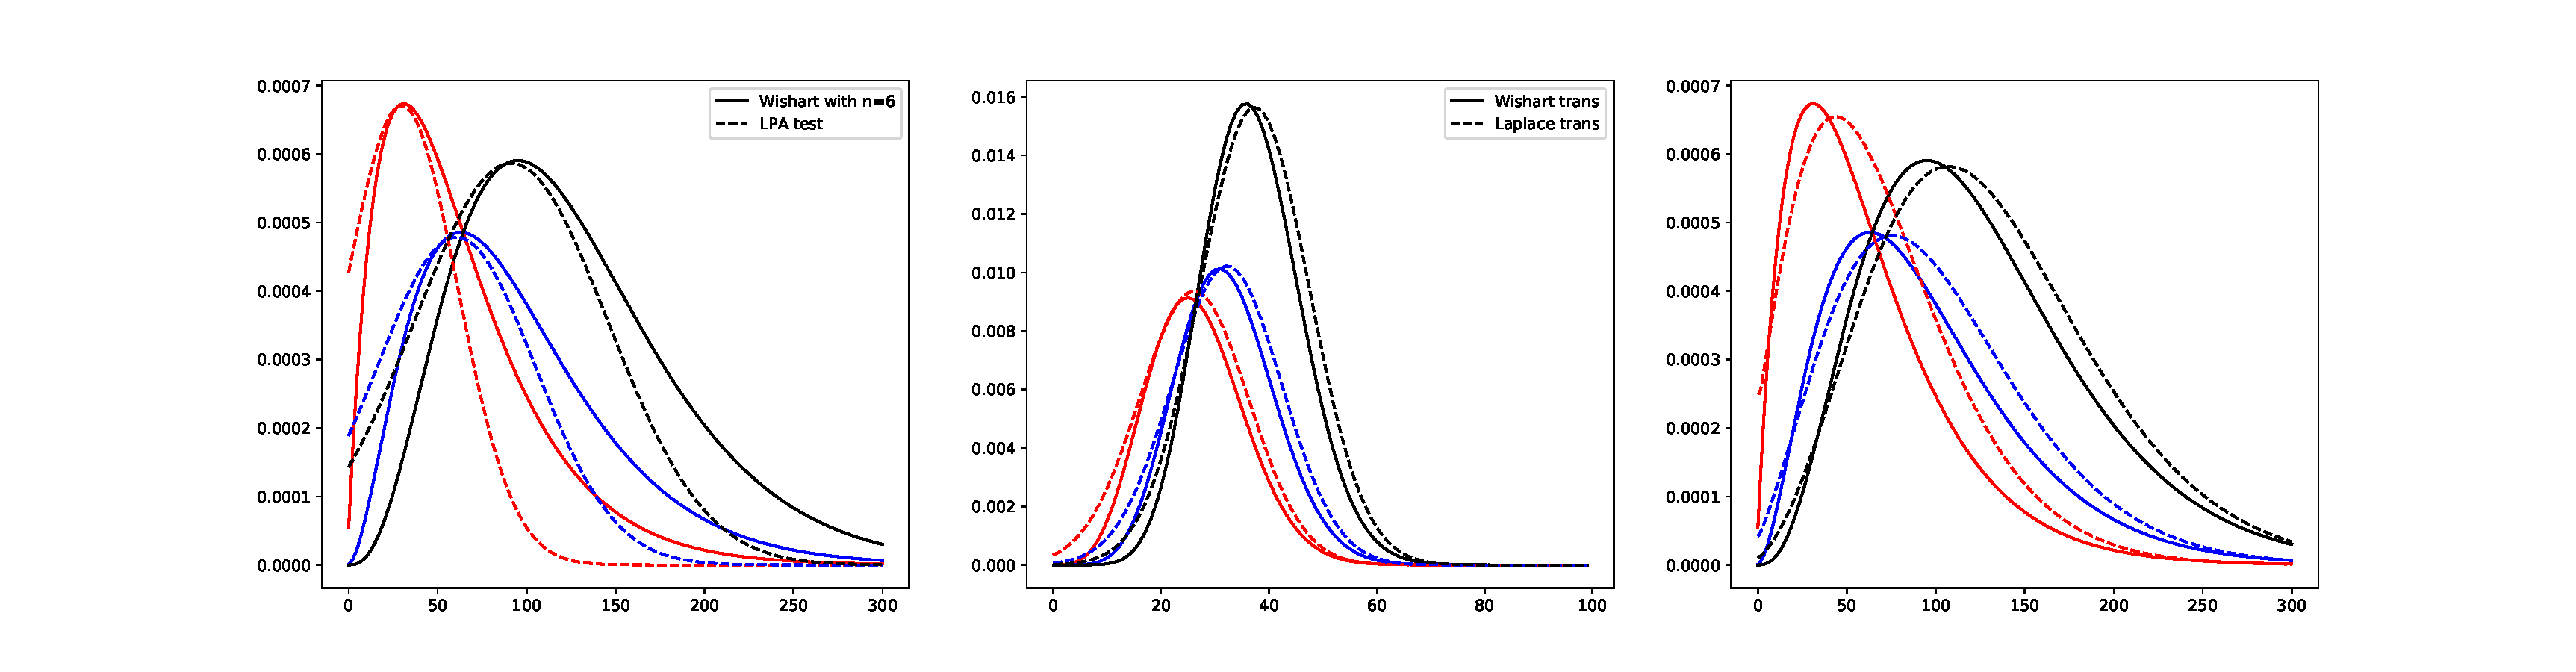
\includegraphics[width=\textwidth]{figures/wishart_playground_sqrtm.pdf}
	\caption{wishart comparison for sqrtm}
	\label{fig:wishart_comparison}
\end{figure}


